\newpage
\chapter{Umsetzung}

\section{Übersicht}

Abbildung \ref{fig:component-overview} zeigt eine grobe Übersicht der wichtigsten Komponenten und deren Verbindungen untereinander. Dieses Design orientiert sich an der Kommunikationsarchitektur, die in Kapitel \ref{sec:communication-architecture} beschrieben ist.

\begin{figure}[H]
	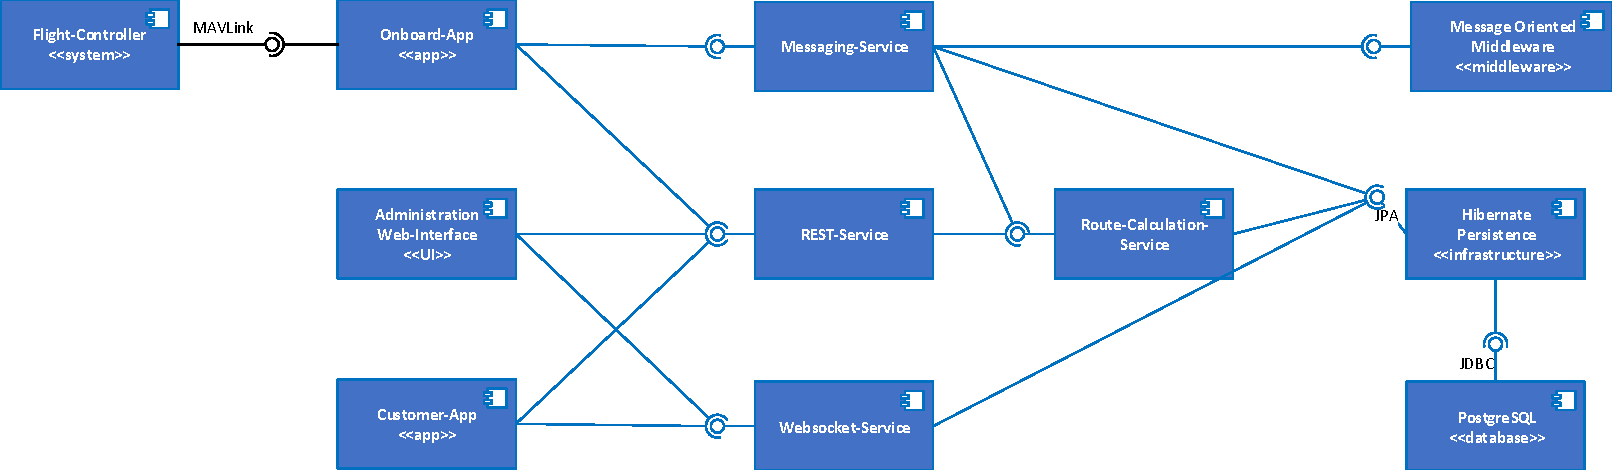
\includegraphics[width=1.0\textwidth]{images/component-overview.pdf}
	\caption{Übersicht der wichtigsten Schnittstellen und deren Verbindungen }
	\label{fig:component-overview}
\end{figure}
\section{Implementierung}

\subsection{Message Broker}
In der Architektur wurde festgelegt, dass der Server und die Onboard-App über Messaging kommunizieren. Um dies zu implementieren, wollten wir einen eigenen Broker auf unserem Server verwenden, um möglichst unabhängig von kostenpflichtigen Cloud-Anbietern zu sein. \\

Ein geeigneter Message Broker muss sowohl vom Server als auch von der Onboard-App angesprochen werden können. Diese Anforderung verunmöglicht den Einsatz von allen \Gls{JMS}-kompatiblen Message Brokern, da \Gls{JMS} nicht mit der Android Plattform kompatibel ist. Als plattformunabhängige Alternative, kommt somit nur ein \Gls{AMQP}-fähiger Broker in Frage. Dafür stehen zwar mehrere Produkte zur Auswahl, aber nur RabbitMQ kann den Broker und alle Client-Bibliotheken liefern.\\

\subsection{Server}

\subsubsection{Play Framework}
Für eine Anwendung in diesem Umfang ist der De-Facto-Standard SpringMVC. Da Spring aber ein schwergewichtiges Framework ist und wir eine neuere, leichtgewichtigere Alternative in der Praxis evaluieren wollten, haben wir uns für das Play Framework entschieden.\\

Zusätzliche Gründe die unsere Entscheidung für Play unterstützt haben:

\begin{itemize}
    \item Fortschrittlicher O/R-Mapper im Framework integriert
    \item Vorgegebene MVC-Architektur (speziell geeignet für \Gls{CRUD}-Operationen)
    \item Schnelle Implementation durch Spezialisierung auf diese Anwendungsart 
    \item Alle Entwickler des Projekts sind versiert in Java
    \item RabbitMQ Anbindung möglich
    \item WebSocket Anbindung möglich
\end{itemize}

\subsubsection{Kommunikation mit den Drohnen}

Um die Möglichkeit zu haben mit einzelnen Drohnen zu kommunizieren, müssen auf dem Server zur Laufzeit alle Verbindungen zu allen Drohnen bekannt sein. Ausserdem muss es möglich sein, eingehende Nachrichten an einem zentralen Punkt abzuarbeiten. Aufgrund der bestehenden MVC-Struktur der Play-Applikation haben wir uns entschieden, auch die Nachrichten aus dem Messaging-System in Controllern zu behandeln, wie es normalerweise nur mit HTTP-Requests geschieht.\\

Die Abbildung \ref{fig:drone-communication-diagram} zeigt ein Objekt-Diagramm von Instanzen, welche die Kommunikation mit den Drohnen erlauben, sobald die Applikation gestartet ist.

\begin{figure}[H]
	\centering
	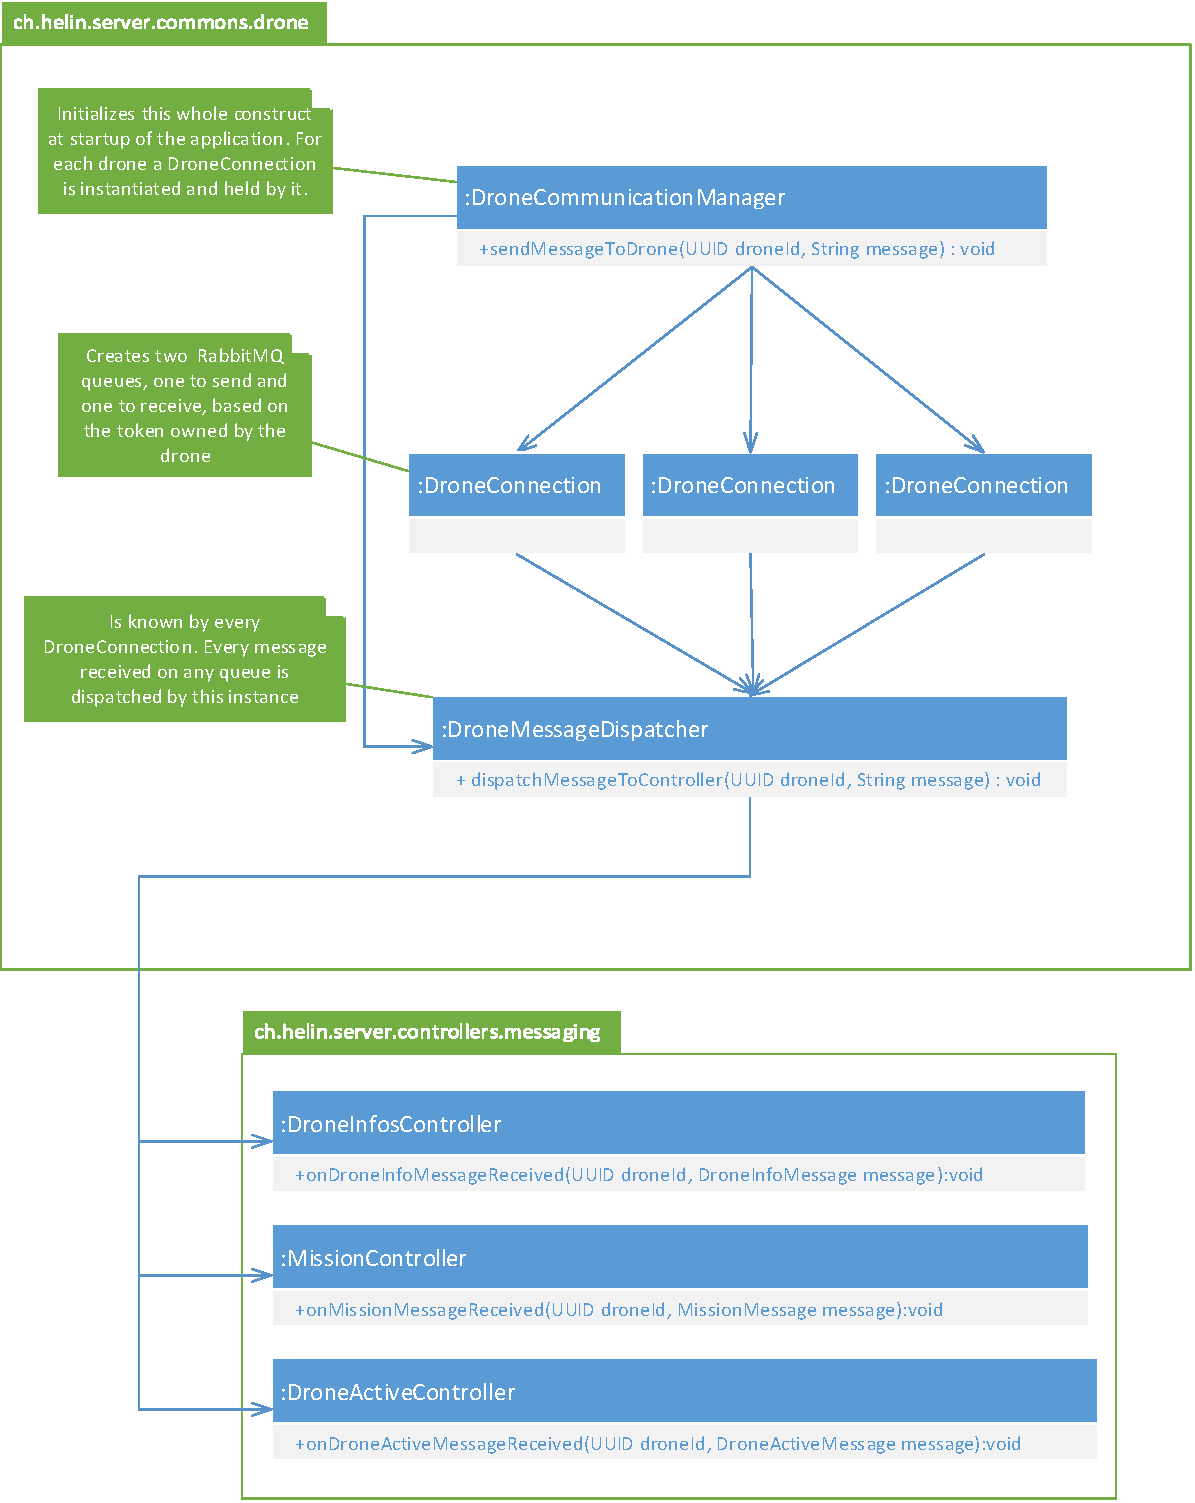
\includegraphics[width=0.8\paperwidth] {images/drone-communication-diagram.pdf}
	\caption{Objekt-Diagramm der Kommunkationsstruktur}
	\label{fig:drone-communication-diagram}
\end{figure}

\subsubsection{Verwendete Bibliotheken}


\begin{tabularx}{\textwidth}{|l|X|l|X|}
	\hline
	\textbf{Name} & \textbf{Verwendungszweck} & \textbf{Version} & \textbf{Lizenz} \\
	\hline \hline
	Hibernate ORM Mapper & objekt-relationales Mapping zwischen Datenbank und Java Objekten  & 5.1.0 & Apache 2.0\\
	\hline 
	RabbitMQ Client & Client Komponente zur Kommunikation mit dem Rabbit MQ Broker & 3.6.0 &  Mozilla Public License 1.1, GPL 2, Apache 2.0 \\
	\hline 
	jGraphT & Graph-Bibliothek für Java, um effizient Operationen auf dem Graph auszuführen & 0.9.2 &  LGPL, EPL \\
	\hline 
\end{tabularx} \\

Bemerkungen aus der Evaluation oben stehender Komponenten:
\begin{itemize}
	\item{\textbf{Hibernate ORM Mapper:} Hibernate ORM ist der einzige ORM Mapper, der eine Spatial-Extension anbietet. Durch Hibernate Spatial ist es möglich, PostGIS Objekte aus der Datenbank direkt zu Java Objekten zu konvertieren.}
	\item{\textbf{RabbitMQ Client:} Als Message Broker wurde auf RabbitMQ gesetzt, daher wurde konsequenterweise RabbitMQ Client als Bibliothek verwendet.}
	\item{\textbf{jGraphT:} Hibernate Spatial arbeitet mit der Java Topology Suite (\Gls{JTS}) zur Abbildung der geografischen Daten. Um aus \Gls{JTS} Objekten einen Graphen zu bilden, kann nur jGraphT verwendet werden.}
\end{itemize}

\subsection{Onboard-App}

\subsubsection{Entwicklungsumgebung}
Um den \Gls{Flight-Controller} mit \Gls{MAVLink} ansprechen zu können, musste eine Android/Java Library gefunden werden, die dies ermöglicht. Die Firma 3DR, der Hersteller des Pixhawk \Gls{Flight-Controller}s, stellt dafür eine Open Source Android-API bereit. Die API kann im App integriert werden und erlaubt es, dem \Gls{Flight-Controller} direkt Befehle zu erteilen. Ausserdem kann man über diese Schnittstelle auch Telemetriedaten auslesen und Events handeln, z.B. Höhenänderungen. Damit war es möglich, die Drohne vom App und damit auch vom Server aus zu steuern.\\

Um während der Entwicklung laufend Tests durchzuführen, ohne jedes Mal mit der echten Drohne zu testen, verwendeten wir eine Software, die den \Gls{Flight-Controller} simuliert. Die Simulation verhält sich nahezu identisch wie ein richtiger Controller und hilft herauszufinden, ob die gesendeten Befehle die erwartete Wirkung zeigen. \\

Die verschiedenen Möglichkeiten, das System zu testen sind im Github Repository dokumentiert. In der Abbildung \ref{fig:test-setup-onboard} wird ein Setup gezeigt, bei dem die Onboard-App im Android Emulator läuft (rechts unten). Gleichzeitig zeigt die Bodenstationssoftware die Echtzeit-Daten des simulierten Fluges an.

\begin{figure}[H]
	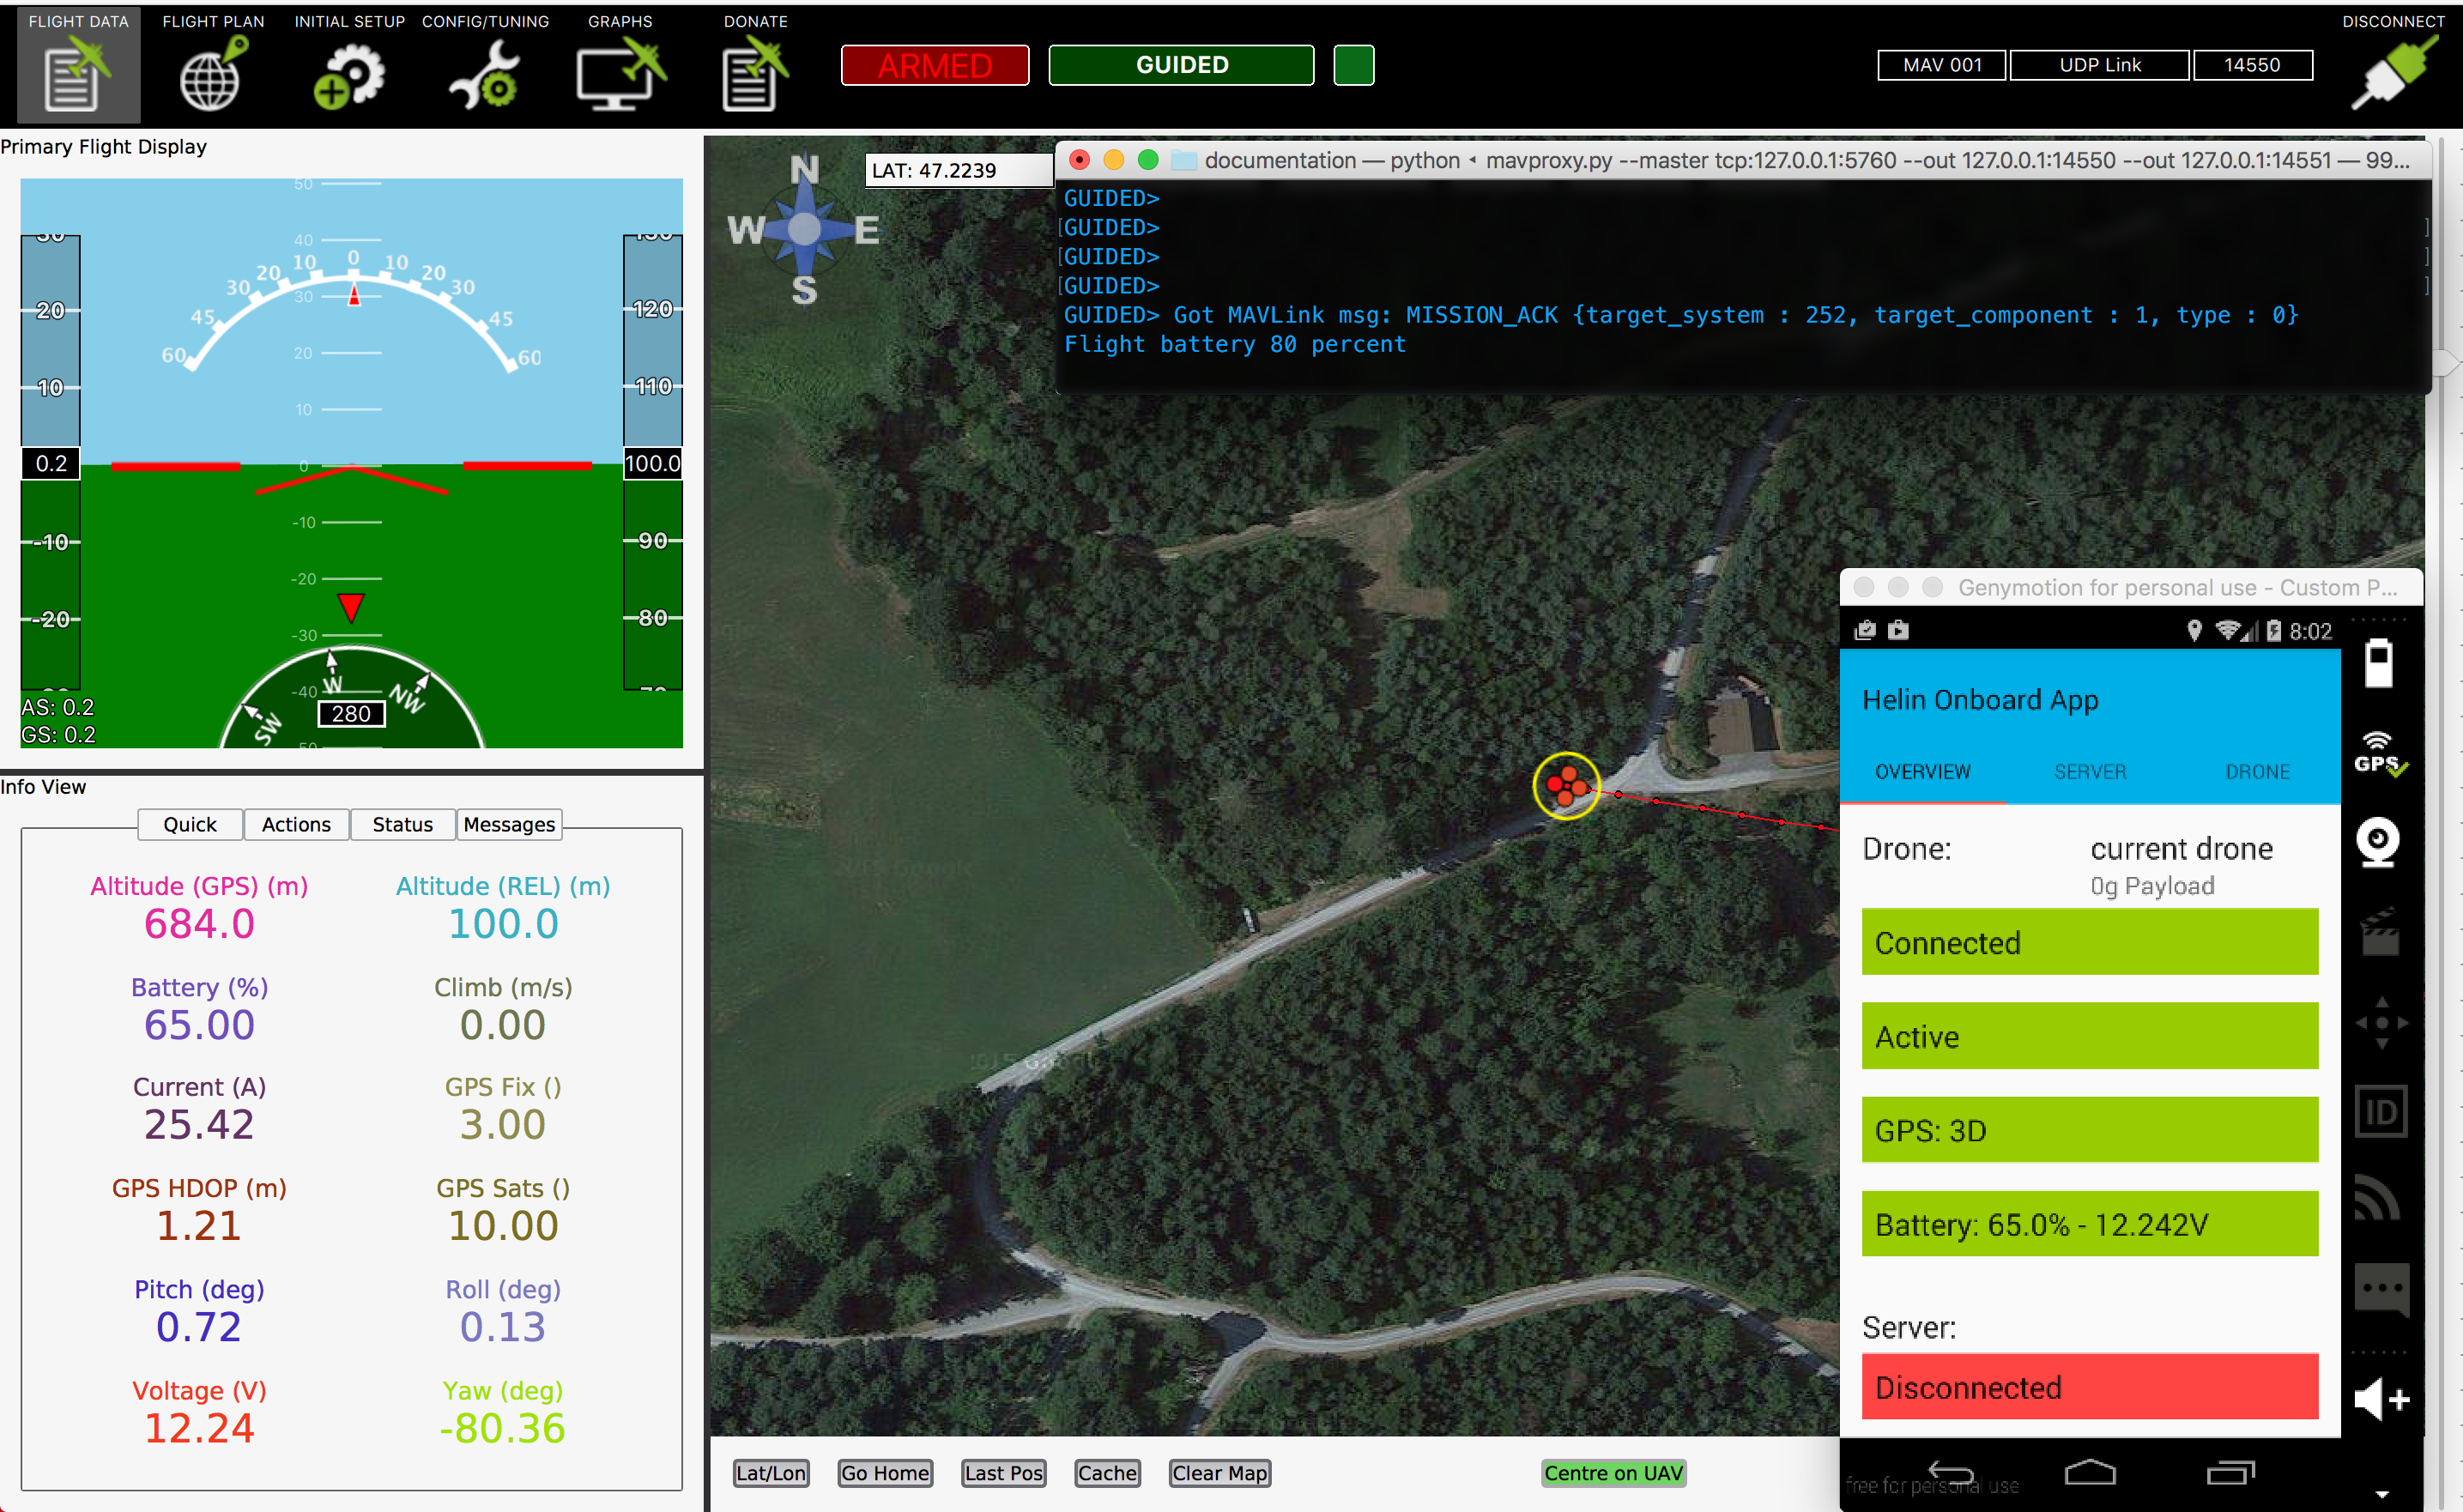
\includegraphics[width=1.0\textwidth]{images/test-setup-onboard.png}
	\caption{APM Planner 2.0 als Bodenstation und Android Emulator mit Onboard App}
	\label{fig:test-setup-onboard}
\end{figure}

\subsubsection{Verwendete Bibliotheken}
\begin{tabularx}{\textwidth}{|X|X|c|X|}
	\hline
	\textbf{Name} & \textbf{Verwendungszweck} & \textbf{Version} & \textbf{Lizenz} \\
	\hline \hline
	DroneKit-Android Client & Android API für \Gls{MAVLink} Protokoll zum ansteuern der Drohne & 1.5.1 & Apache 2.0\\
	\hline 
	AMQP Messaging Library & Messaging für Android & 3.6.0 &  Mozilla Public License 1.1, GPL 2,  Apache 2.0 \\
	\hline 
	Lyra  & High availability Messaging & 0.4.3 &  Apache 2.0 \\
	\hline 
	Dagger  & Dependency Injection Framework für Android & 2.0.1 &  Apache 2.0 \\
	\hline 
\end{tabularx} \\

Bemerkungen aus der Evaluation oben stehender Komponenten:
\begin{itemize}
	\item{\textbf{DroneKit-Android Client:} Es existiert keine gleichwertige Alternative die das \Gls{MAVLink} Protokoll in diesem Umfang abdeckt.}
	\item{\textbf{Lyra:} Die Bibliothek wird vom Hersteller der Message-Oriented-Middleware (\Gls{MOM}) empfohlen. \cite[]{lyra-page} }
	\item{\textbf{AMQP Messaging Library:} Ermöglicht den Zugriff auf den RabbitMQ Message Broker.}
	\item{\textbf{Dagger:} Wird von Google entwickelt und unterstützt Dependency Injection zur Kompilierzeit.}
\end{itemize}

\subsubsection{Kommunikation zum Server}

Gemäss den nicht-funktionalen Anforderungen soll ein Verbindungsabbruch zum Server keinen Einfluss auf die Ausführung der Lieferung haben. Deshalb wird die Flugroute vor dem Start auf den \Gls{Flight-Controller} übertragen, somit kann die Mission auch ohne Online-Verbindung erfolgreich abgeschlossen werden. \\

Sollte die Verbindung zwischen Server und Onboard-App unterbrochen sein, sollte verhindert werden, dass Nachrichten verloren gehen. Bei unterbrochener Verbindung wird dies wie folgt erreicht:
\begin{itemize}
	\item{\textbf{Nachricht vom Server zum Onboard-App} \\
		Dieses Szenario wird durch RabbitMQ abgefangen. Der Message Broker persistiert die Nachrichten solange bis die Onboard-App wieder verfügbar ist. Es besteht somit kein zusätzlicher Handlungsbedarf.
	}
	\item{\textbf{Nachricht vom Onboard-App an den Server} \\
		Hier steht der Message Broker nicht zur Verfügung und die Speicherung der Nachrichten musste implementiert werden. Dazu verwenden wir eine Queue in der alle Nachrichten gespeichert werden und erst entfernt werden, wenn sie verschickt wurden.
	}
\end{itemize}
Mit diesen Massnahmen haben wir eine gute Balance zwischen Zuverlässigkeit und Implementationsaufwand erreicht.



\subsubsection{Verbindungswiederherstellung}
Gemäss den nicht-funktionalen Anforderungen, muss sichergestellt werden, dass nach einem Unterbruch der Internetverbindung eine Verbindungswiederherstellung stattfindet. Sobald die Verbindung mit dem Internet wieder besteht, soll nach 30 Sekunden wieder eine Verbindung zum Message Broker bestehen. \\

Bei der Konfiguration der Verbindungswiederherstellung bestand die Wahl zwischen fixen oder inkrementellen Zeitabständen, nach denen eine Wiederherstellung versucht wird. Um das exakte Verhalten zu evaluieren, wurden Versuche gemacht, bei denen die Verbindung für drei Sekunden unterbrochen wurde (siehe Tabelle \ref{tbl:backoff}).\\

\begin{table}
	
	\centering
	\begin{tabular}{|r|r|r|}
		\hline
		\textbf{Versuch} & \textbf{Mit inkrementellem Intervall [s] } & \textbf{Mit fixem Intervall [s]} \\
		\hline
		1 & 17 & 7 \\
		2 &	7 & 7 \\
		3 & 9 & 7 \\
 		4 & 11 & 7 \\
		5 & 10 & 7 \\
		\hline
	\end{tabular}
	\caption{Benötigte Zeit für Verbindungswiederherstellung}
	\label{tbl:backoff}
\end{table}

Da beide Varianten die nicht-funktionalen Anforderungen erfüllen, haben wir uns nach den Versuchen für ein inkrementelles Intervall entschieden, um das Smartphone nicht unnötig zu belasten.

\subsection{Customer App}
Gemäss Aufgabenstellung sollte ein Prototyp für eine App, mit welchem Bestellungen am System abgegeben können, entwickelt werden.

Anders als die Onboard-App, welche native mit Java entwickelt wurde und nur auf Android läuft, entschieden wir uns beim Customer-App für eine Cross-Plattform Lösung, welche Android und iOS unterstützt. \\

Auch wenn gemäss der Aufgabenstellung keine iOS-App gefordert war, stellte sich doch die Frage ob man die iPhone-Kunden ausschliessen soll und spätere Entwickler zwingt, einen grossen Teil des Codes in einer nativen iOS App duplizieren zu müssen. Mit einem Marktanteil von 42.2\% (Zahlen 2015) \cite{ios-user} von iOS Benutzern in der Schweiz, ist anzunehmen, dass zu einem späteren Zeitpunkt eine iPhone App implementiert werden muss.\\

Deshalb wurde auf Xamarin Forms gesetzt, welches ermöglicht, die ganzen Service-Klassen und einen Teil der Benutzeroberfläche für die verschiedenen Plattformen nur einmal zu implementieren.

Die App wurde in einer minimalen Ausbaustufe erstellt, erfüllt aber bereits alle nötigen funktionalen Anforderungen. In Abbildung \ref{fig:customer-app-flow} wird gezeigt, wie ein Benutzer durch die App navigieren kann. 

Besonders wichtig ist die Anzeige des berechneten Abwurfpunktes vor der Bezahlung der Bestellung, sowie die Anzeige der Drohnenposition während des Anflugs.  

\begin{landscape}
	\begin{figure}[h]
		\centering
		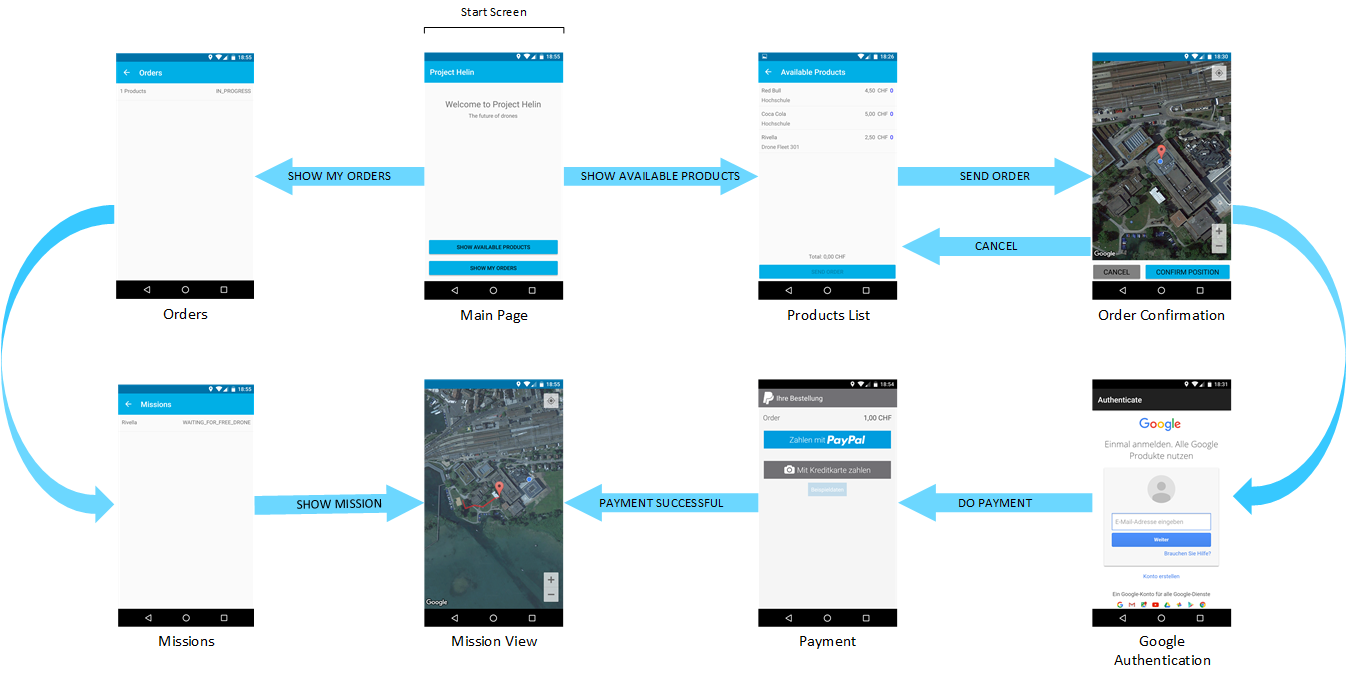
\includegraphics[width=0.8\paperheight] {images/customer-app-pages.png}
		\caption{Übersicht der Customer-App mit allen Verknüpfungen zwischen den Screens}
		\label{fig:customer-app-flow}
	\end{figure}
\end{landscape}

\subsubsection{Verwendete Bibliotheken}
\begin{tabularx}{\textwidth}{|X|X|c|X|}
	\hline
	\textbf{Name} & \textbf{Verwendungszweck} & \textbf{Version} & \textbf{Lizenz} \\
	\hline \hline
	PayPal Forms & PayPal Integration für Xamarin.Forms & 2.0.4 & MIT \\
	\hline 
	Xamarin Forms & Plattformübergreifende Komponente für Xamarin & 2.2.0.45 & \url{https://www.xamarin.com/license} \\
	\hline 
	Websocket.PCL & Plattformübergreifende WebSocket Anbindung & 1.1.9 & MIT \\
	\hline 
	Newton.Json & Json zu Object mapper & 8.0.3 & MIT \\
	\hline 
\end{tabularx}\\

Bemerkungen aus der Evaluation oben stehender Komponenten:
\begin{itemize}
	\item{\textbf{PayPal Forms:} Einziges PayPal Plugin für Xamarin.Forms}
	\item{\textbf{Xamarin.Forms:} Ermöglicht Crossplattform UI, sehr einfach zu entwickeln}
	\item{\textbf{Websocket.PCL:} Einzige gut gewartete Implementation von WebSockets in Xamarin}
	\item{\textbf{Newton.Json:} Die Bibliothek weist die höchste Anzahl Downloads auf}
\end{itemize}

\subsection{Datenbank}

Die Anforderungen an das Datenbank Management System (\Gls{DBMS}) für dieses Projekt, können wie folgt zusammengefasst werden:

\begin{itemize}
	\item Geobasierte Objekte abzuspeichern muss möglich sein (Speicherung von Zonen)
	\item Anbindung an das Play-Framework muss möglich sein
\end{itemize}

Es gibt zwei ausgereifte Produkte, die diese Anforderungen erfüllen: Oracle mit Oracle-Spatial und PostgreSQL mit PostGIS. Bei Oracle-Spatial und PostGIS handelt es sich um Erweiterungen, die im DMBS eingebunden werden können und es ermöglichen, geobasierte Daten abzuspeichern und spezialisierte Abfragen darauf auszuführen. \\

Die Entscheidung zu Gunsten von PostgreSQL wurde getroffen, da zwei Teammitglieder bereits Erfahrungen mit dem System vorweisen können und es sich, wie bei unserem Projekt, um eine Open Source Software handelt. \\

Zusätzlich wurde für PostGIS die Erweiterung \Gls{SFCGAL} verwendet, welche die Geometriebibliothek \Gls{CGAL} in PostGIS verfügbar macht. Dies ermöglicht noch weitere Funktionen in der Datenbank zu nutzen, welche auf geometrischen Objekten ausgeführt werden können.

\subsection{Sicherheit}
Es ist essentiell, dass die Sicherheit bei der Kommunkation zwischen Server und Drohne gewährleistet ist, da sonst die Kontrolle über eine Drohne übernommen werden könnte (siehe NFR \ref{sec:message-security}). Um diese Sicherheit zu gewährleisten wurde ein Prozess eingeführt, der es ermöglicht die Zugangsdaten für den RabbitMQ Message Broker und die Queue-Namen geheim zu halten: \\

Die Onboard-App registriert sich über einen HTTPS Request beim Server. Bei erfolgreicher Registrierung der Drohne, wird ein Token sowie der Benutzer und das Kennwort für die Verbindung zu RabbitMQ an die Onboard-App geschickt. Mit diesen Informationen kann sich die App mit dem Messaging Broker über eine verschlüsselte Leitung verbinden.\\

Für die darauf folgende Kommunikation mit dem Broker, werden mit Hilfe des Tokens zwei Queues erzeugt: 
\begin{itemize}
	\item \{token\}-Drone-To-Server
	\item \{token\}-Server-To-Drone
\end{itemize}

Über diese Queues können jetzt Nachrichten ausgetauscht werden. \\

Ein Angreifer müsste mit dieser Methode den Token herausfinden und auch die Zugangsdaten für den Broker kennen, um mit einer Drohne zu kommunizieren. Falls jemand es aber doch schaffen würde, die Benutzerdaten auszulesen, gibt es trotzdem noch $2^{122}$ mögliche Tokens, die durchprobiert werden müssten. \\

\section{Projektgrösse}

Folgende Statistiken wurden am Ende der Arbeit erstellt um einen Eindruck der Grösse des Projekts zu erhalten.\\
\begin{table}[H]
	\begin{tabularx}{\textwidth}{|X|r|r|r|r|}
		\hline
		\textbf{Metrik} & \textbf{Server} & \textbf{Onboard-App} & 
		\textbf{Customer-App} & \textbf{Total} \\
		\hline
		\hline
		\textbf{Lines of Code} & 12071 & 2174 & 1188 & 15433 \\
		\hline
		\textbf{Anteil Lines of Code Tests} & 29.34\% & 13.58\% & 0.00\% & 24.85\% \\
		\hline
		\textbf{Anteil Lines of Code Kommentare} & 4.03\% & 1.33\% & 0.00\% & 3.18\% \\
		\hline
		\textbf{Anzahl Klassen} & 174 & 49 & 36 & 259 \\
		\hline
		\textbf{Anzahl Methoden mit hoher \mbox{zyklomatischer} Komplexität} & 1.73\% & 1.57\% & N/A & 1.46\% \\
		\hline
	\end{tabularx}
	\caption{Code Metriken nach Abschluss der Arbeit}
	\label{table:code-metrics}
\end{table}

In der Tabelle \ref{table:code-metrics} sind vor allem der geringe Anteil von Methoden mit hoher essentieller Komplexität\cite[]{MCCABE} hervorzuheben. Alle Methoden mit hoher Komplexität wurden vom Team geprüft, konnten aber nicht mehr verbessert werden. Hauptsächlich sind dies 'equals' Methoden von grösseren \Gls{DTO}s oder es handelt sich um MessageConverter, die einfach alle verschiedenen Messagetypen verschieden behandeln müssen. Das folgende Beispiel zeigt die Methode mit der höchsten zyklomatischen Komplexität der Server-Applikation (Essentielle Komplexität = 10, Zyklomatische Komplexität = 10). \\


\begin{lstlisting}
private Message parseMessageWithoutCare(String messageAsJson) {
	...
	switch (payloadType) {
		case ConfirmCargoLoaded:
			return gson.fromJson(messageAsJson, ConfirmCargoLoaded.class);
		case NotifyCargoDrop:
			return gson.fromJson(messageAsJson, NotifyCargoDrop.class);
		case DroneInfo:
			return gson.fromJson(messageAsJson, DroneInfoMessage.class);
		case DroneDto:
			return gson.fromJson(messageAsJson, DroneDtoMessage.class);
		case AssignMission:
			return gson.fromJson(messageAsJson, AssignMissionMessage.class);
		case FinalAssignMission:
			return gson.fromJson(messageAsJson, FinalAssignMissionMessage.class);
		case ConfirmMission:
			return gson.fromJson(messageAsJson, ConfirmMissionMessage.class);
		case FinishedMission:
			return gson.fromJson(messageAsJson, FinishedMissionMessage.class);
		case DroneActiveState:
			return gson.fromJson(messageAsJson, DroneActiveStateMessage.class);
	}
}

\end{lstlisting}

Da diese Methode gut strukturiert ist und auch gut verstanden werden kann, gibt es keinen Grund, diese auf Grund der Metrik anzupassen.

\newpage
\section{Qualitätssicherung}
\label{quality-assurance}

\subsection{Prozesse}

Zur Qualitätssicherung wurde im Projektmanagement-Tool neben Todo, In Progress und Done ein neuer Quality-Assurance-Status für die Issues eingeführt. Alle Issues in diesem Status mussten von einem anderen Teammitglied überprüft werden, bevor sie auf Done geschoben werden konnten. \\

Die Überprüfung eines Issues beinhaltet folgende Aufgaben:

\begin{itemize}
	\item{Akzeptanzkriterien aus der User-Story manuell prüfen}
	\item{Code-Review durchführen (Intensität je nach Grösse und Komplexität des geschriebenen Codes)}
	\item{Code auf Vertösse gegen Style-Guide prüfen}
	\item{Prüfen der Tests vorhanden sind}
\end{itemize}

Damit konnten viele Fehler früh entdeckt werden und die Code-Qualität konnte über die ganze Projektdauer konstant gehalten werden.

\subsection{Continous Integration}

Als Build-Server haben wir TeamCity verwendet. Dort sind alle Projekte (ausser Customer-App) jeweils mit einem Build für den develop- und master-branch eingerichtet. Alle Builds führten die Tests aus und produzierten ein entsprechendes Artifact für das Deployment. Das Deployment für den Server wurde ebenfalls automatisiert.

\subsection{Testing}

Je nach Plattform wurden andere Formen von Tests durchgeführt:

\subsubsection{Server}

Auf dem Server wurden vor allem \Gls{E2E-Test}s und \Gls{Integration-Test}s verwendet, um die Funktionalität zu prüfen. Wir haben uns bei den meisten Kompoonenten bewusst gegen \Gls{Unit-Tests} entschieden, da auf dem Server nur wenig Logik zu finden ist, die nicht von der Datenbank oder der RabbitMQ-Connection abhängt. Unit-Tests hätten deswegen nur einen ganz kleinen Teil der Anwendungen abdecken können und wären in den meisten Fällen sehr aufwendig gewesen. Bei der Routenberechnung hingegen konnte sehr gut mit Unit-Tests gearbeitet werden.\\

Wir haben darauf geachtet, dass immer nur die minimale Integrationsstufe gewählt wurde. Für die Simulation eines Benutzers (E2E) wurde Selenium verwendet, das wiederum einen Firefox Browser verwendet. Für die Api- und Messaging-Controller wurden Integrationtests verwendet, welche keinen Browser benötigen.\\

Es wurde eine \textbf{durchschnittliche Testabdeckung von 72\%} über das ganze Projekt erreicht. In wichtigen Packages liegt diese aber meist über 85\%.

\subsubsection{Onboard-App}

Beim Onboard App wurden nur Unit-Tests ausgeführt. Der Aufbau von E2E Tests ist denkbar, hätte den Rahmen dieser Arbeit aber gesprengt. Deshalb wurden hauptsächlich die Message-Handler und die Daten-Mapper getestet. Diese haben eine \textbf{Testabdeckung von 86\%}.

\subsubsection{Customer-App}

Bei der Customer-App wurden keine Tests eingerichtet, da es sich um einen Prototypen handelt.


